\documentclass{beamer}
\usepackage[utf8]{inputenc}

\usetheme{Boadilla}
\usecolortheme{lily}
\usepackage{amsmath,amssymb,amsfonts,amsthm}
\usepackage{mathtools}
\usepackage{txfonts}
\usepackage{tkz-euclide}
\usepackage{listings}
\usepackage{adjustbox}
\usepackage{array}
\usepackage{tabularx}
\usepackage{lmodern}
\usepackage{gvv}
\usepackage[T1]{fontenc}
\usepackage{circuitikz}
\usepackage{tikz}
\usepackage{graphicx}

\setbeamertemplate{footline}
{
  \leavevmode%
  \hbox{%
  \begin{beamercolorbox}[wd=\paperwidth,ht=2.25ex,dp=1ex,right]{author in head/foot}%
    \insertframenumber{} / \inserttotalframenumber\hspace*{2ex} 
  \end{beamercolorbox}}%
  \vskip0pt%
}

\usepackage{tcolorbox}
\tcbuselibrary{minted,breakable,xparse,skins}




\providecommand{\nCr}[2]{\,^{#1}C_{#2}} % nCr
\providecommand{\nPr}[2]{\,^{#1}P_{#2}} % nPr
\providecommand{\mbf}{\mathbf}
\providecommand{\pr}[1]{\ensuremath{\Pr\left(#1\right)}}
\providecommand{\qfunc}[1]{\ensuremath{Q\left(#1\right)}}
\providecommand{\sbrak}[1]{\ensuremath{{}\left[#1\right]}}
\providecommand{\lsbrak}[1]{\ensuremath{{}\left[#1\right.}}
\providecommand{\rsbrak}[1]{\ensuremath{{}\left.#1\right]}}
\providecommand{\brak}[1]{\ensuremath{\left(#1\right)}}
\providecommand{\lbrak}[1]{\ensuremath{\left(#1\right.}}
\providecommand{\rbrak}[1]{\ensuremath{\left.#1\right)}}
\providecommand{\cbrak}[1]{\ensuremath{\left\{#1\right\}}}
\providecommand{\lcbrak}[1]{\ensuremath{\left\{#1\right.}}
\providecommand{\rcbrak}[1]{\ensuremath{\left.#1\right\}}}
\theoremstyle{remark}
\renewcommand{\sgn}{\mathop{\mathrm{sgn}}}
\renewcommand{\solution}{\noindent\textbf{Solution: }}
\providecommand{\abs}[1]{\left\vert#1\right\vert}
\providecommand{\res}[1]{\Res\displaylimits_{#1}} 
\providecommand{\norm}[1]{\lVert#1\rVert}
\providecommand{\mtx}[1]{\mathbf{#1}}
\providecommand{\mean}[1]{E\left[ #1 \right]}
\providecommand{\fourier}{\overset{\mathcal{F}}{ \rightleftharpoons}}
%\providecommand{\hilbert}{\overset{\mathcal{H}}{ \rightleftharpoons}}
\providecommand{\system}{\overset{\mathcal{H}}{ \longleftrightarrow}}
	%\newcommand{\solution}[2]{\textbf{Solution:}{#1}}
%\newcommand{\solution}{\noindent \textbf{Solution: }}
\providecommand{\dec}[2]{\ensuremath{\overset{#1}{\underset{#2}{\gtrless}}}}
\let\vec\mathbf

\lstset{
%language=C,
frame=single, 
breaklines=true,
columns=fullflexible
}

\numberwithin{equation}{section}

\lstset{
  language=Python,
  basicstyle=\ttfamily\small,
  keywordstyle=\color{blue},
  stringstyle=\color{orange},
  numbers=left,
  numberstyle=\tiny\color{gray},
  breaklines=true,
  showstringspaces=false
}

\title{Problem 2.10.47}
\author{EE25BTECH11018-Darisy Sreetej}

\date{\today} 
\begin{document}

\begin{frame}
\titlepage
\end{frame}


\section{Problem}

\begin{frame}
\frametitle{Problem}
The value of $a$ so that the volume of parallelopiped formed by $\hat{i} + a\hat{j} + \hat{k}, \hat{j} + a\hat{k} \text{ and } a\hat{i} + \hat{k}$ becomes minimum is
\begin{enumerate}
\item $-3$
\item $3$
\item $\frac{1}{\sqrt{3}}$
\item $\sqrt{3}$
\end{enumerate}
\end{frame}
%\subsection{Literature}
\section{Solution}

\subsection{Formula}
\setcounter{section}{1}
\begin{frame}
\frametitle{Formula}
Volume of the parallelopiped
\begin{align*}
 V=\vec{p} \cdot (\vec{q} \times \vec{r}) 
\end{align*}
\end{frame}
\subsection{Obtaining Volume}
\begin{frame}
\frametitle{Obtaining Volume}
The Volume of the parallelopiped formed by $\vec{p},\vec{q},\vec{r}$ is ,
\begin{align}
    V = \vec{p}\cdot(\vec{q}\times\vec{r})
\end{align}
\begin{align}
V=\mydet{
    1 && a && 1\\
    0 && 1 && a\\
    a && 0 && 1
    }
\end{align}
\begin{align}
    V=a^3-a+1
\end{align}


\end{frame}
\subsection{Finding a for minimum volume}
\begin{frame}[fragile]
\frametitle{Finding 'a' for minimum volume}
    Now , consider
\begin{align}
    f(a)=a^3-a+1\\
    f'(a)=3a^2+1
\end{align}
\begin{align*}
\text{Set }f'(a)=0  \Rightarrow a^2=\frac{1}{\sqrt{3}} \Rightarrow a=\frac{1}{\sqrt{3}} or -\frac{1}{\sqrt{3}} 
\end{align*}
\begin{align}
\text{Second derivative }f''(a)=6a\\
\text{At }a=\frac{1}{\sqrt{3}},f''>0 \Rightarrow minimum\\
\text{At }a=-\frac{1}{\sqrt{3}},f''<0 \Rightarrow maximum
\end{align}
Therefore , $a=\frac{1}{\sqrt{3}}$ for which the Volume of the parallelopiped becomes minimum.
\end{frame}
\subsection{Plot}
\begin{frame}[fragile]
\frametitle{Plot}

\begin{figure}[h!]
   \centering
   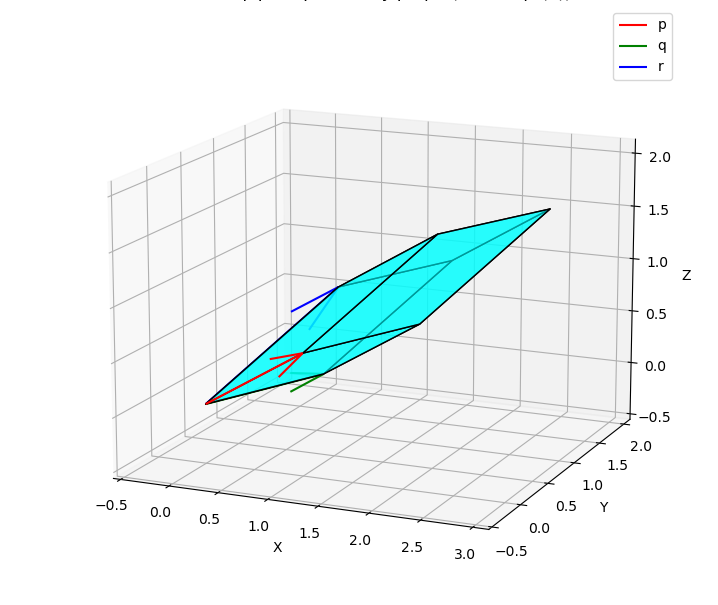
\includegraphics[width=0.7\columnwidth]{figs/fig.png}
	\caption{Parallelopiped with Vectors $\vec{p},\vec{q},\vec{r}$ for which $a=\frac{1}{\sqrt{3}}$(Volume is minimum)}
    \label{}
\end{figure}
\end{frame}

\section{C Code}
\begin{frame}[fragile]
\frametitle{C Code}
\begin{lstlisting}[language=C]
#include <stdio.h>
#include <math.h>
// Function to calculate determinant of 3x3 matrix
double determinant(double a) {
    double mat[3][3] = {
        {1, a, 1},
        {0, 1, a},
        {a, 0, 1}
    };
    double det = mat[0][0]*(mat[1][1]*mat[2][2] - mat[1][2]*mat[2][1])
               - mat[0][1]*(mat[1][0]*mat[2][2] - mat[1][2]*mat[2][0])
               + mat[0][2]*(mat[1][0]*mat[2][1] - mat[1][1]*mat[2][0]);

    return det; }
    \end{lstlisting}
\end{frame}
\begin{frame}[fragile]
    \frametitle{C code}
    \begin{lstlisting}[language=C]
// Function f(a) = a^3 - a + 1
double f(double a) {
    return (a*a*a - a + 1);
}
// Function to check if a given 'a' is a local minimum
int isLocalMinimum(double a) {
    double secondDerivative = 6*a;
    return (secondDerivative > 0); // local min if f''(a) > 0
}
int main() {
    double options[4] = {-3, 3, 1.0/sqrt(3), sqrt(3)};
    int i;

    printf("Checking all options:\n");
    \end{lstlisting}
\end{frame}
\begin{frame}[fragile]
    \frametitle{C code}
    \begin{lstlisting}[language=C]
  for (i = 0; i < 4; i++) {
        double a = options[i];
        double vol = determinant(a);

        printf("a = %lf, Determinant = %lf, f(a) = %lf", a, vol, f(a));

        if (fabs(a - 1.0/sqrt(3)) < 1e-6 && isLocalMinimum(a)) {
        
        printf("\n");
    }
    printf("\nTherefore, the local minimum occurs at a = 1/sqrt(3).\n");
    return 0;
}
     \end{lstlisting}
\end{frame}
\section{Python Code}
\begin{frame}[fragile]
\frametitle{Python Code for Solving}
\begin{lstlisting}[language=Python]
import ctypes
import math
# Load the compiled shared library
lib = ctypes.CDLL("./volume.so")

# Declare function signatures
lib.determinant.argtypes = [ctypes.c_double]
lib.determinant.restype = ctypes.c_double
lib.f.argtypes = [ctypes.c_double]
lib.f.restype = ctypes.c_double
lib.isLocalMinimum.argtypes = [ctypes.c_double]
lib.isLocalMinimum.restype = ctypes.c_int

# Options to check
options = [-3, 3, 1.0/math.sqrt(3), math.sqrt(3)]
print("Checking all options:\n")
\end{lstlisting}
\end{frame}
\section{Python Code}
\begin{frame}[fragile]
\frametitle{Python Code for Solving}
\begin{lstlisting}[language=Python]
for a in options:
    det_val = lib.determinant(a)
    f_val = lib.f(a)
    is_min = lib.isLocalMinimum(a)
    print(f"a = {a:.6f}, Determinant = {det_val:.6f}, f(a) = {f_val:.6f}", end="")
print("\nTherefore, the local minimum occurs at a = 1/sqrt(3).")
\end{lstlisting}
\end{frame}
\begin{frame}[fragile]
\frametitle{Python Code for Plotting}
\begin{lstlisting}[language=Python]
import numpy as np
import matplotlib.pyplot as plt
from mpl_toolkits.mplot3d.art3d import Poly3DCollection

# Define vectors for a = 1/sqrt(3)
a = 1/np.sqrt(3)
p = np.array([1, 0, a])
q = np.array([a, 1, 0])
r = np.array([1, a, 1])

# Parallelepiped vertices (8 corners)
O  = np.array([0, 0, 0])     # origin
P  = p
Q  = q
R  = r
PQ = p + q
PR = p + r
QR = q + r
PQR = p + q + r
\end{lstlisting}
\end{frame}
\begin{frame}[fragile]
\frametitle{Python Code for Plotting}
\begin{lstlisting}[language=Python]
vertices = [O, P, Q, PQ, R, PR, QR, PQR]

# Faces of parallelepiped (each face is a list of 4 vertices)
faces = [
    [O, P, PQ, Q],
    [O, P, PR, R],
    [O, Q, QR, R],
    [P, PQ, PQR, PR],
    [Q, PQ, PQR, QR],
    [R, PR, PQR, QR]
]

# Plot
fig = plt.figure(figsize=(8, 8))
ax = fig.add_subplot(111, projection='3d')

# Draw faces
ax.add_collection3d(Poly3DCollection(faces, facecolors='cyan', 
                                     edgecolors='black', alpha=0.6))

\end{lstlisting}
\end{frame}
\begin{frame}[fragile]
\frametitle{Python Code for Plotting}
\begin{lstlisting}[language=Python]
# Draw vectors p, q, r
ax.quiver(0, 0, 0, *p, color='r', label='p')
ax.quiver(0, 0, 0, *q, color='g', label='q')
ax.quiver(0, 0, 0, *r, color='b', label='r')

# Set limits
all_points = np.array(vertices)
ax.set_xlim([np.min(all_points[:,0])-0.5, np.max(all_points[:,0])+0.5])
ax.set_ylim([np.min(all_points[:,1])-0.5, np.max(all_points[:,1])+0.5])
ax.set_zlim([np.min(all_points[:,2])-0.5, np.max(all_points[:,2])+0.5])
ax.set_xlabel("X")
ax.set_ylabel("Y")
ax.set_zlabel("Z")
ax.set_title("Parallelopiped formed by p, q, r (a = 1/sqrt(3))")
ax.legend()
plt.show()
\end{lstlisting}
\end{frame}
\end{document}